\documentclass[14pt, a4paper]{article}

%%%%%%%%%% Математика %%%%%%%%%%
\usepackage{amsmath,amsfonts,amssymb,amsthm,mathtools}
%\mathtoolsset{showonlyrefs=true}  % Показывать номера только у тех формул, на которые есть \eqref{} в тексте.
%\usepackage{leqno} % Нумерация формул слева

%%%%%%%%%%%%%%%%%%%%%%%% Шрифты %%%%%%%%%%%%%%%%%%%%%%%%%%%%%%%%%
\usepackage{fontspec}         % пакет для подгрузки шрифтов
\setmainfont{Linux Libertine O}       % задаёт основной шрифт документа

% why do we need \newfontfamily:
% http://tex.stackexchange.com/questions/91507/
\newfontfamily{\cyrillicfonttt}{Linux Libertine O}
\newfontfamily{\cyrillicfont}{Linux Libertine O}
\newfontfamily{\cyrillicfontsf}{Linux Libertine O}
% Иногда тех не видит структуры шрифтов. Эти трое бравых парней спасают ситуацию и доопределяют те куски, которые Тех не увидел.

\usepackage{unicode-math}     % пакет для установки математического шрифта
\setmathfont{Asana Math}      % шрифт для математики

\usepackage{polyglossia}      % Пакет, который позволяет подгружать русские буквы
\setdefaultlanguage{russian}  % Основной язык документа
\setotherlanguage{english}    % Второстепенный язык документа

%%%%%%%%%% Работа с картинками %%%%%%%%%
\usepackage{graphicx}                  % Для вставки рисунков
\usepackage{graphics}
\graphicspath{{images/}{pictures/}}    % можно указать папки с картинками
\usepackage{wrapfig}                   % Обтекание рисунков и таблиц текстом
\usepackage{float}

%%%%%%%%%% Оформление %%%%%%%%%%
\usepackage{extsizes} % Возможность сделать 14-й шрифт
% размер листа бумаги
\usepackage[paper=a4paper,top=10mm, bottom=10mm,left=35mm,right=35mm,includefoot,includehead]{geometry}

\usepackage{setspace}
\setstretch{1}  % Межстрочный интервал
\setlength{\parindent}{0pt} % Красная строка.
\setlength{\parskip}{4mm} % Между абзацами.



\usepackage{titlesec}  

% В Linux этот пакет сделан косячно. Исправляет это следующий непонятный кусок кода. 
\makeatletter
\patchcmd{\ttlh@hang}{\parindent\z@}{\parindent\z@\leavevmode}{}{}
\patchcmd{\ttlh@hang}{\noindent}{}{}{}
\makeatother

\titleformat{\section}
	 {\bfseries\Large}
	 {\thesection:}{0.5 em}{}

\renewcommand{\thesection}{Приложение~\Asbuk{section}}

\renewcommand{\labelitemi}{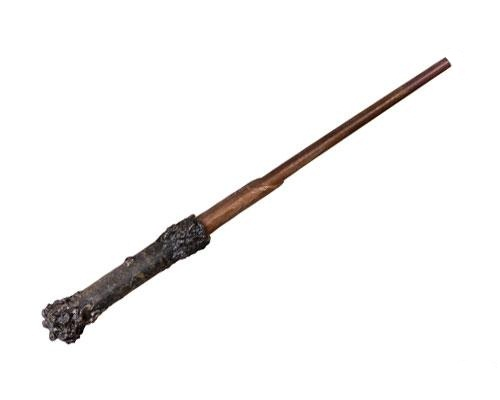
\includegraphics[scale=0.05]{wizard.jpg}}


\usepackage{fancyhdr} % Колонтитулы
\pagestyle{fancy}

\renewcommand{\headrulewidth}{0.2pt}  % Толщина линий, отчеркивающих верхний
\fancyhead[L]{\leftmark}
\fancyhead[R]{\thepage}
\fancyfoot{ } 
\fancyfoot[C]{Школа Чародейства и Волшебства «Хогвартс»}     

\begin{document}

\thispagestyle{empty}

\begin{figure}[H]
\begin{center}

\includegraphics[height=6cm]{hogwarts.png}
\end{center}
\end{figure}

\vspace{1cm}

{\fontsize{12}{1}\selectfont Мистеру Поттеру}

\vspace{2.5cm}

Дорогой мистер Поттер,

Мы рады проинформировать вас, что вам предоставлено место в Школе Чародейства и Волшебства «Хогвартс».

Пожалуйста, ознакомьтесь с приложенным к данному письму списком необходимых книг и предметов.

Занятия начинаются 1 сентября. Ждем вашу сову не позднее 31 июля.


\vfill

Искренне ваша,

{\fontspec{Always In My Heart} \fontsize{26}{1}\selectfont \hspace{3mm} Minerva Mc gonagall }

Минерва МакГонагалл \\
заместитель директора

\vspace{10mm}

\begin{center}
Школа Чародейства и Волшебства «Хогвартс» \\
\vspace{2mm}
\small Директор: Альбус Дамблдор \\
(Кавалер ордена Мерлина первой степени, основатель Ордена \\ Феникса, председатель Международной Конфедерации Магов)
\end{center} 

\newpage 

\section{Список необходимых книг и предметов} 

\begin{itemize}
\item Волшебная палочка
\item Мантия-невидимка
\item Камень, оживляющий мёртвых
\item Задачник Демидовича
\end{itemize}

\newpage
 
\section{ Список изучаемых предметов} 

\begin{itemize}
\item Трансфигурация
\item История магии
\item Математический анализ
\end{itemize}


\end{document}
